\section{Information Visualization II}
\subsection{Visual Encoding}
Le visualizzazioni sono composte da \textbf{marks} (segnali) e 
\textbf{channels} (canali). I marks sono gli oggetti grafici che rappresentano gli elementi di dati (ad esempio, punti, linee, barre).
I channels sono le proprietà grafiche che rappresentano gli attributi dei dati (ad esempio, colore, posizione, forma, dimensione).


La codifica visiva significa passare dai dati alle rappresentazioni visive.
La codifica richiede non solo la scelta di un grafico appropriato per i dati in questione (tipo e semantica),
ma anche la selezione degli elementi grafici individuali e delle loro proprietà.

\subsection{Graphical Elements}
\begin{figure}[H]
    \centering
    \begin{minipage}{0.45\textwidth}
        \centering
        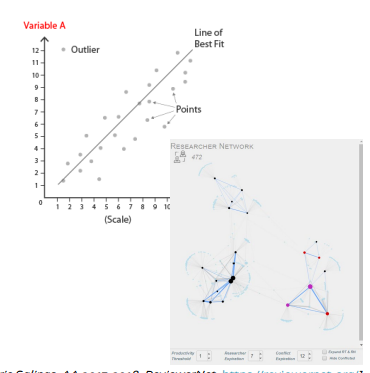
\includegraphics[width=\linewidth]{images/Marks.png} 
        \caption{Esempio di Marks}
        \label{fig:immagine1}
    \end{minipage}\hfill
    \begin{minipage}{0.45\textwidth}
        \centering
        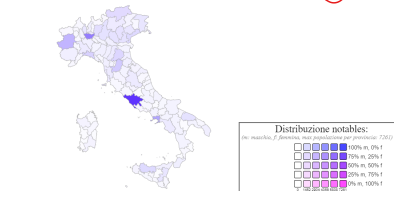
\includegraphics[width=\linewidth]{images/Channels.png} % Sostituisci 'immagine2' con il nome del tuo file immagine
        \caption{Esempio di Channels}
        \label{fig:immagine2}
    \end{minipage}
\end{figure}
Le componenti contestuali sono elementi che rendono più semplice interpretare le visualizzazioni.
Un esempio sono: le labesls, annotazioni, legende, griglie, assi cartesiani.
\begin{figure}[H]
    \centering
    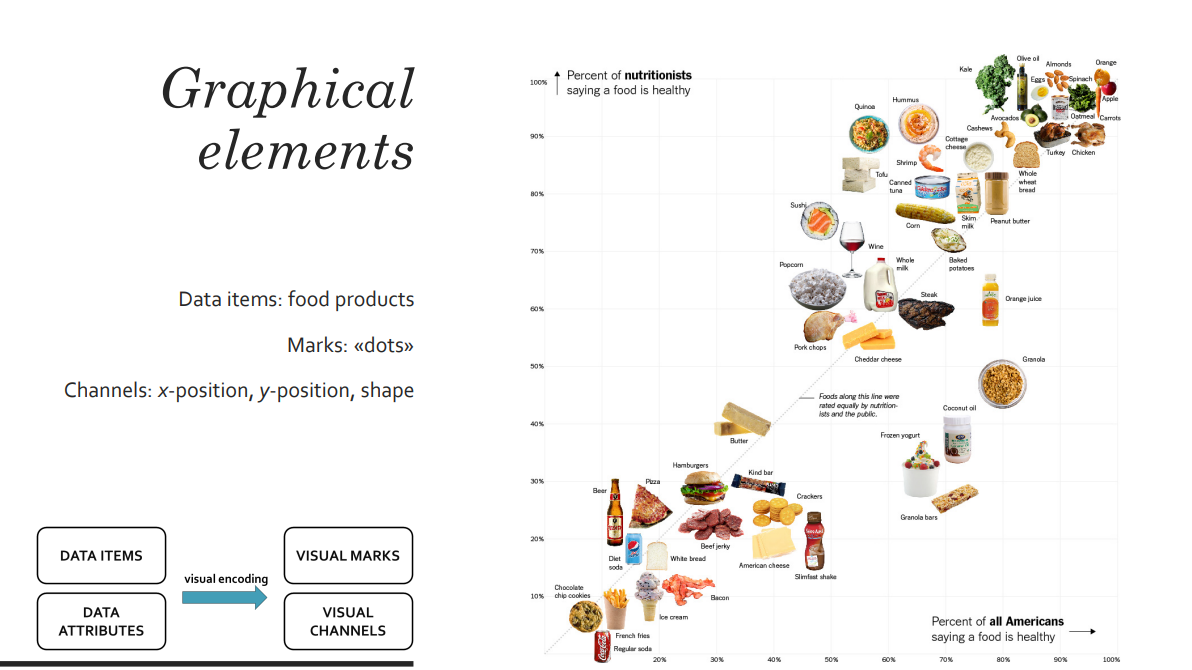
\includegraphics[width=0.5\textwidth]{images/CompleteExMC.png} % Sostituisci 'nome_immagine' con il nome del tuo file immagine
    \caption{Esempio completo di Channels e Marks di un grafico}
    \label{fig:immagine}
\end{figure}
\subsection{Visual decoding}
\begin{figure}[H]
    \centering
    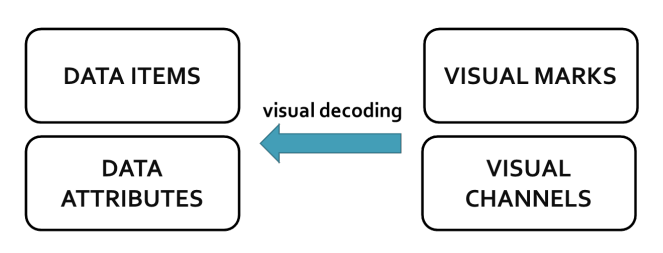
\includegraphics[width=0.5\textwidth]{images/VisDec.png} % Sostituisci 'nome_immagine' con il nome del tuo file immagine
    \caption{Visual Decoding}
    \label{fig:immagine}
\end{figure}
Per \textbf{Visual Decoding} si intende destrutturare una rappresentazione visiva nei suoi principali elementi e identificare:
\begin{itemize}
    \item gli elementi grafici, quali sono i segnali visivi? Quali sono i canali visivi?
    \item le regole di mappatura (ossia, le informazioni che i singoli elementi grafici rappresentano)
        quali elementi di dati rappresentano i segnali? Quali attributi rappresentano i canali?
\end{itemize}
È utile per valutare e ridisegnare le visualizzazioni.

\begin{figure}[H]
    \centering
    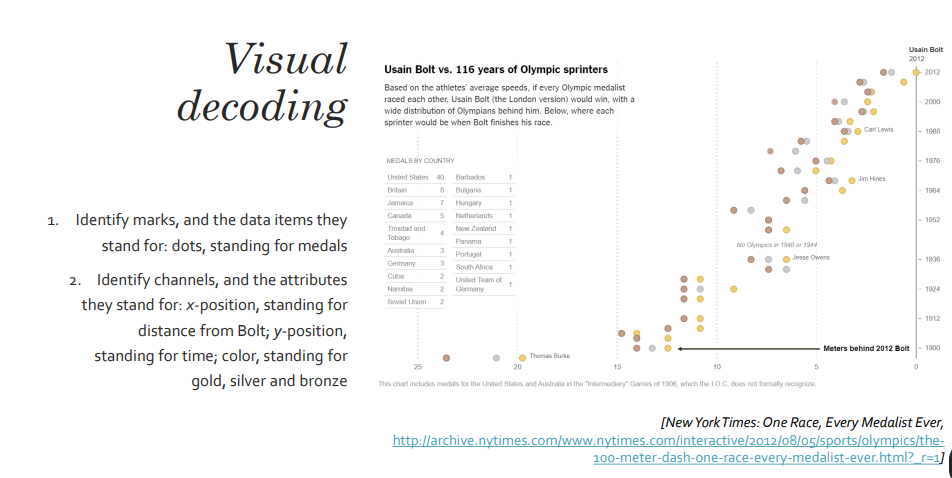
\includegraphics[width=0.5\textwidth]{images/ExComplDec.png} % Sostituisci 'nome_immagine' con il nome del tuo file immagine
    \caption{Esempio completo di Decoding}
    \label{fig:immagine}
\end{figure}

\subsubsection{Quality Evaluation}
La valutazione di una visualizzazione può basarsi su due principi 
guida principali: \textbf{Expressiveness} ed \textbf{Effectiveness}.
\textbf{Expressiveness}: la Visual representation dovrebbe rappresentare tutte e solo le relazioni che esistono nei dati.
Le informazioni rilevanti dovrebbero essere prioritarie e quindi codificate con i canali più efficaci/accurati.
\begin{figure}[H]
    \centering
    \begin{minipage}{0.45\textwidth}
        \centering
        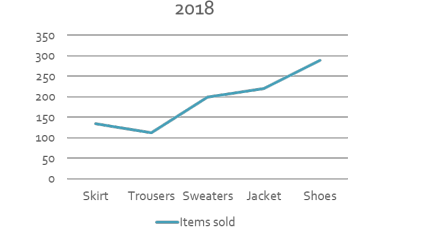
\includegraphics[width=\linewidth]{images/ErroreEff.png} 
        \caption{Dati non ordinati che sembrano ordinati (nell'esempio seguente, stiamo mostrando informazioni su un trend che non è nei dati:
         la forma della linea non ha significato).}
        \label{fig:immagine1}
    \end{minipage}\hfill
    \begin{minipage}{0.45\textwidth}
        \centering
        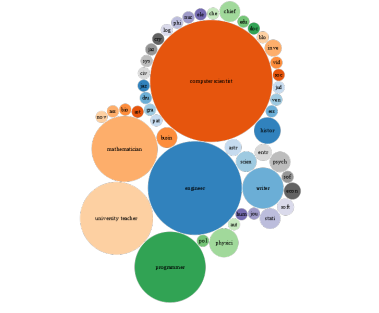
\includegraphics[width=\linewidth]{images/ErroreEff2.png} % Sostituisci 'immagine2' con il nome del tuo file immagine
        \caption{utilizzo dei colori quando non restituiscono alcuna informazione}
        \label{fig:immagine2}
    \end{minipage}
\end{figure}
\subsubsection{Percentuale di Accuracy}
Quanto sono efficaci i canali nel trasmettere diversi tipi di attributi?
Uno dei (possibili) riassunti per attributi quantitativi.
\begin{figure}[H]
    \centering
    \begin{minipage}{0.45\textwidth}
        \centering
        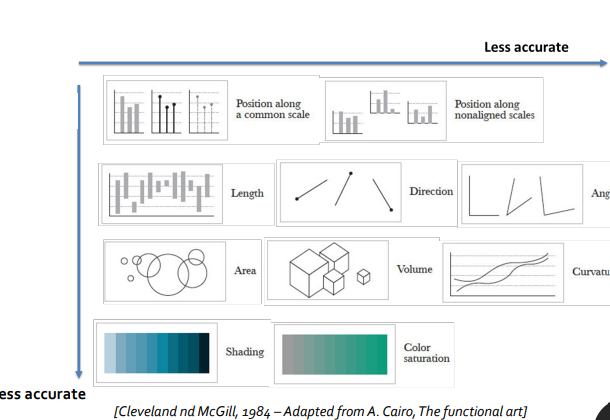
\includegraphics[width=\linewidth]{images/percentAcc1.png} 
        \caption{Riassunto dell'accuracy di ogni grafico.}
        \label{fig:immagine1}
    \end{minipage}\hfill
    \begin{minipage}{0.45\textwidth}
        \centering
        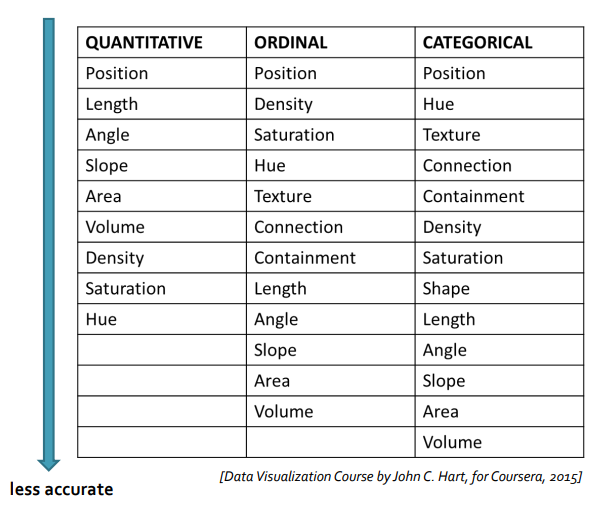
\includegraphics[width=\linewidth]{images/percentAcc2.png} 
        \caption{Riassunto dell'accuracy di ogni grafico}
        \label{fig:immagine2}
    \end{minipage}
\end{figure}
\subsection{Altri tipi di grafici}
\subsubsection{WordClouds}
Rappresentazione di quanto frequentemente le parole appaiono in un determinato corpo di testo attraverso la dimensione della parola
Variazioni nell'arrangiamento e nel colore
Principalmente utilizzato per motivi estetici.
\begin{figure}[H]
    \centering
    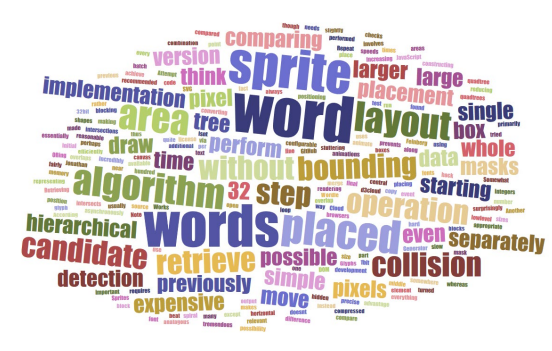
\includegraphics[width=0.5\textwidth]{images/WordClouds.png} 
    \caption{WordClouds}
    \label{fig:immagine}
\end{figure}
\subsubsection{Calligrams}
Testi disposti in modo tale da formare un'immagine tematicamente correlata.
L'immagine creata dalle parole illustra il testo esprimendo visivamente qualcosa associato (o in contrasto) a ciò che il testo dice.
\begin{figure}[H]
    \centering
    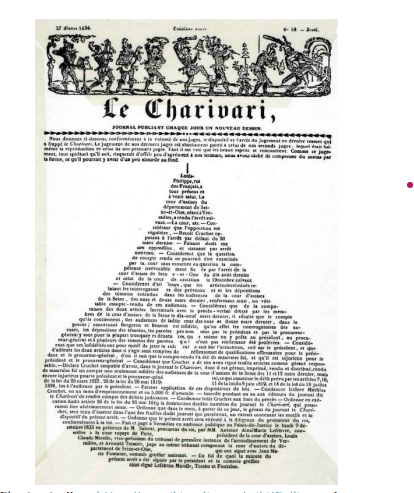
\includegraphics[width=0.5\textwidth]{images/Calligrams.png} 
    \caption{Calligrams}
    \label{fig:immagine}
\end{figure}

\subsubsection{Flow Maps}

Raffigurare il movimento delle entità posizionando linee tracciate sopra delle mappe (spazio e tempo)
Lo spessore, il colore, ecc. possono codificare informazioni aggiuntive
In questa mappa: dimensioni delle truppe, distanza percorsa, temperatura, latitudine e longitudine, direzione del viaggio, tempo.
\begin{figure}[H]
    \centering
    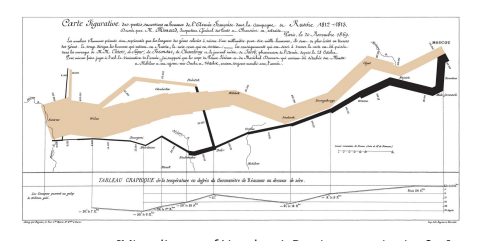
\includegraphics[width=0.5\textwidth]{images/FlowMaps.png}
    \caption{Flow Maps}
    \label{fig:immagine}
\end{figure}
\subsubsection{Chernoff faces}
Ragionamento: siamo molto bravi nel riconoscere i volti.
Introdotto da Herman Chernoff nel 1973
Variabili sono mappate su tratti del viso
(larghezza/curvatura della bocca, dimensione verticale del viso, dimensione/inclinazione/separazione degli occhi, dimensione delle sopracciglia, posizione verticale delle sopracciglia…)
\begin{figure}[H]
    \centering
    \includegraphics[width=0.5\textwidth]{images/Chernofffaces.png} 
    \caption{Chernoff faces}
    \label{fig:immagine}
\end{figure}
\subsubsection{Multidimensional Icons}
Spence e Parr (1991) proposero di codificare le proprietà di un oggetto in una semplice rappresentazione tramite icone. 
Hanno applicato questo approccio per verificare le offerte di permanenza.
\begin{figure}[H]
    \centering
    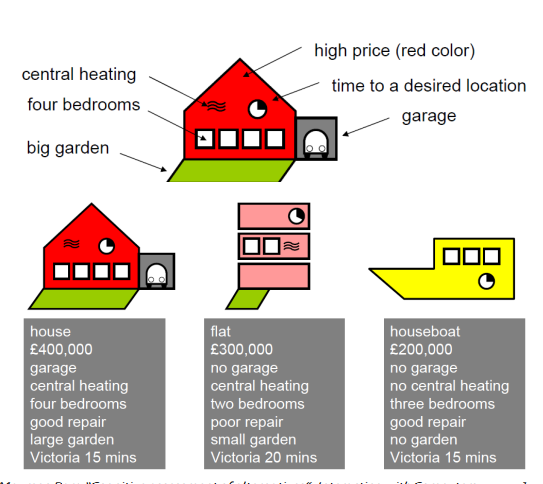
\includegraphics[width=0.5\textwidth]{images/MultiIcon.png} 
    \caption{Multidimensional Icons}
    \label{fig:immagine}
\end{figure}
\subsubsection{Petal as a gliph}
L'idea di Moritz Stefaner per visualizzare un indice di vita consiste nel mappare diverse variabili (relative alle condizioni di vita materiale e alla qualità della vita) in petali di diverse dimensioni, per confrontare il benessere tra paesi.
\begin{figure}[H]
    \centering
    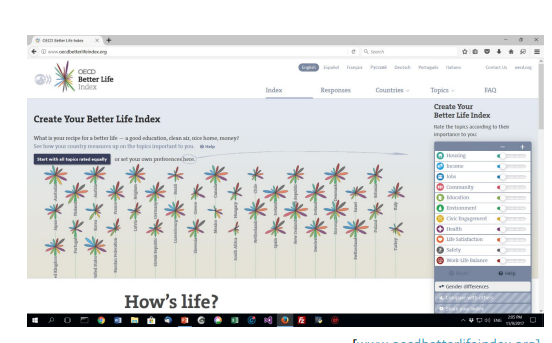
\includegraphics[width=0.5\textwidth]{images/PetalGliph.png} 
    \caption{Petal as a gliph}
    \label{fig:immagine}
\end{figure}
